% *==================================================================================*
% *                     Review vs. Camera-Ready settings                             *
% *==================================================================================*
%
% REVIEW: Use the following command for submitting the paper (double-blind,
% for review):
% \documentclass{Interspeech}
%
% CAMERA-READY: Use the following command for the camera-ready version, one
% affiliation per line:
\documentclass[cameraready]{Interspeech}
%\documentclass{Interspeech}
% *==================================================================================*


\title{BACON: Boundary-Aware Convolution for Streaming Conformer Models}

\author{Hainan}{Xu}
\author{Kunal}{Dhawan}
\author{Dongji}{Gao} 
\author{Jagadeesh}{Balam}

\address{
    NVIDIA Corporation
}

\email{hainanx@nvidia.com}

\keywords{streaming speech recognition, conformer, boundary-aware convolution, chunk-based processing}

\newcommand{\blue}[1]{\textcolor{blue}{#1}}
\newcommand{\red}[1]{\textcolor{red}{#1}}
\usepackage{comment}

\begin{document}
\maketitle

%----------------------------------------------------------------------
\begin{abstract}
We propose \emph{Boundary-Aware CONvolution} (BACON), a drop-in replacement for causal convolution in streaming sequence tasks that leverage chunk-based Conformers.
These streaming Conformers typically pair chunked attention with
causal convolution to prevent future information from crossing chunk
boundaries. We show that
causal convolution is unnecessarily restrictive: within a chunk, all frames
are already available, so the convolution kernel can safely look ahead up to
the chunk boundary without violating the streaming constraint.
BACON exploits
this by splitting the depthwise convolution channels into a causal group and a
boundary-aware bidirectional group, yielding a wider effective receptive field
than the causal baseline while preserving parameter count.
Across single-speaker Automatic Speech Recognition (ASR), multi-speaker ASR, and speech-to-text translation tasks with two model architectures,
BACON improves model accuracy while maintaining comparable latency.

\end{abstract}

%----------------------------------------------------------------------
\section{Introduction}
\label{sec:intro}

Real-world speech applications (e.g., voice assistants, real-time captioning,
and simultaneous translation) typically require \emph{streaming} processing:
instead of waiting for the complete input audio, the model produces outputs
incrementally as
audio arrives, within a bounded latency budget. 
Among streaming architectures,
\emph{chunk-based} models~\cite{chen2021developing} accumulate a short window
of frames before processing them as a unit, trading a small fixed delay for
richer within-window acoustic context than fully frame-to-frame causal approaches.

The Conformer~\cite{gulati2020conformer,rekesh2023fast} is a prominent architecture in modern
speech models, combining self-attention~\cite{vaswani2017attention} with
depthwise separable convolutions~\cite{kaiser2017depthwise} which enables the model to capture both global dependencies and local temporal features.
For chunk-based streaming, two standard modifications are typically applied: (1)~\emph{chunked
attention}, which restricts each frame's attention
to prevent access to future chunks, and (2)~\emph{causal convolution}, which
restricts the depthwise kernel to current and past frames only. 
Together, these modifications ensure that model computation does not depend on future chunks.

We argue that the second modification is overly conservative. 
In a chunk-based system, all frames within a chunk are processed together; therefore, a
convolution kernel can look ahead \emph{within the chunk} without violating the
streaming constraint, while causal convolution unnecessarily discards this
available context.



To address this limitation, we propose \emph{Boundary-Aware CONvolution} (BACON), which recovers this wasted within-chunk context. 
BACON splits the depthwise channels into two groups: a \emph{causal} group with full backward context, and a \emph{bidirectional} group whose right context is confined to the current
chunk. 
For convolution with kernel size $k$, the aggregate effective receptive field spans $[-(k-1), (k-1)/2]$, strictly wider than the causal baseline's $[-(k-1), 0]$,
while using the same number of parameters.
The key contributions of this work are:
\begin{itemize}
    \item We identify that causal convolution is unnecessarily strict in
          chunk-based streaming Conformers and that within-chunk look-ahead is
          streaming-safe.
    \item We propose BACON, a split-channel design that widens the effective
          receptive field without breaking chunk-based streaming constraints
          and without adding parameters.
    \item We demonstrate improvements across three tasks
          (single-speaker Automatic Speech Recognition (ASR), multi-speaker ASR, and speech-to-text translation) across two
          model families (\textsc{chat} and \textsc{rnn-t}).
\end{itemize}

\section{Background}
\label{sec:background}

\subsection{Conformer}
\label{subsec:conformer}

The Conformer~\cite{gulati2020conformer} augments the
Transformer~\cite{vaswani2017attention} with depthwise separable convolution.
Each block applies, in order: a feed-forward module, multi-head self-attention,
a convolution module, and a second feed-forward module, with residual
connections and layer normalization throughout. 
The convolution module primarily captures local dependencies, while attention captures broader
dependencies; together they provide complementary representations of the
input~\cite{gulati2020conformer,mohamed2019transformers}.

% The convolution module consists of a pointwise expansion, a gated linear unit
% (GLU)~\cite{dauphin2017language}, a depthwise convolution with kernel
% size~$K$, batch normalization, a Swish activation~\cite{ramachandran2017searching},
% and a pointwise projection. The depthwise convolution determines the temporal
% context each frame can access and is the focus of this work.

\subsection{Chunk-Limited Attention}
\label{subsec:chunk-attention}

In standard self-attention, each frame compares against all frames in the full
input, which is incompatible with streaming. To adapt self-attention for
streaming,
\emph{chunk-limited attention}~\cite{chen2021developing,noroozi2024stateful} partitions
the input into non-overlapping chunks of fixed size and restricts each frame's
attention context to its own chunk and prior chunks. This avoids dependency on
future chunks and enables chunk-wise streaming.

% \begin{equation}
%     \text{Attention}(t) = \text{softmax}\left(\frac{\mathbf{q}_t \mathbf{K}_c^\top}{\sqrt{d_k}}\right)\mathbf{V}_c,
% \end{equation}
% where $\mathbf{K}_c$ and $\mathbf{V}_c$ are the keys and values of chunk~$c$
% and $d_k$ is the key dimension. 
 

\subsection{Causal Convolution}
\label{subsec:causal-conv}

Standard streaming Conformers replace the symmetric depthwise kernel with a
\emph{causal convolution} that sees only current and past frames.
% \begin{equation}
%     y_t = \sum_{i=0}^{K-1} w_i \cdot x_{t-i},
% \end{equation}
%implemented by padding $k{-}1$ zeros on the left with no right padding. 
This
guarantees no future information is accessed and is therefore sufficient for
streaming. However, it is stricter than the chunked streaming constraint requires: in
the chunk-based setting, frames within the same chunk are all available
simultaneously, so right context within the chunk is already present at
processing time.

%----------------------------------------------------------------------
\section{Method}
\label{sec:method}



% \subsection{Within-Chunk Look-Ahead is Streaming-Safe}
% \label{sec:motivation}

% The streaming constraint is that processing frame $t$ must not depend on any
% frame that has not yet been received. In a chunk-based system with chunk
% size~$S$, all frames $\{iS, \ldots, (i{+}1)S{-}1\}$ in chunk~$i$ arrive
% together before processing begins. A convolution applied to chunk~$i$ may
% therefore safely use any frame within chunk~$i$ as context for any other frame
% in the same chunk. Right context that crosses into chunk~$i{+}1$ is forbidden,
% but right context \emph{within} chunk~$i$ is not. Causal convolution discards
% this available context entirely.

Our goal is to allow right-context convolution up to the chunk boundary. A
straightforward approach is to replace causal convolution with a fully
symmetric bidirectional kernel. 
However, near the right boundary of each chunk, the right half of the kernel window falls outside the chunk and must be masked out, reducing effective context size. For example, given a chunk size of $C{=}14$ and a kernel size of 
$k{=}9$, the last four frames of each chunk operate with reduced context. 
To address this, we propose a \emph{dual-context channel design}.

\subsection{Dual-Context Channel Design}
\label{sec:chunk_conv}

We increase convolutional receptive field to the future whenever possible while
preserving past receptive field. This is achieved with a split-channel
design. The $d$ depthwise channels
are divided into two equal groups with different padding strategies:
\begin{itemize}
    \item \textbf{Causal group} ($d/2$ channels): Requires left zero-padding of length $k-1$ only once at the beginning of the utterance. In all other places, it accesses full past context without chunk boundary restrictions.
    \item \textbf{Bidirectional group} ($d/2$ channels): Utilizes a mixed padding strategy with $p=(k-1)/2$. While its left context crosses chunk boundaries freely similar to the causal group; for right context, $p$ zeros is padded at the end of each chunk, to be used for right context of convolutions without breaking chunk boundaries.
\end{itemize}

Since depthwise convolution applies an independent kernel per channel, the two
groups have fully separate learned weights despite residing in the same
convolution module. No parameter sharing occurs between the causal and
bidirectional channels. 

% The combined receptive field is $[-(k-1),\frac{k-1}{2}]$, strictly wider than either
% group alone. For $K{=}9$: the causal group covers $[-8,\;0]$ and the
% bidirectional group covers $[-4,\;+4]$; together they span $[-8,\;+4]$, a
% 13-frame window versus 9 for the causal baseline.



% \subsection{Chunk-Level Processing}
% \label{sec:chunk-processing}

% The causal group is convolved over the full sequence with standard left-only
% padding and requires no chunk-level logic. Processing the bidirectional group
% proceeds per chunk as follows:
% \begin{enumerate}
%     \item \textbf{Extend left}: prepend $P$ frames from the preceding chunk
%           (zero-pad for the first chunk).
%     \item \textbf{Pad right}: append $P$ zeros at the right chunk edge.
%     \item \textbf{Convolve}: apply the depthwise kernel, producing $S$ output
%           frames for the chunk.
%     \item \textbf{Reassemble}: concatenate chunk outputs along the time axis.
% \end{enumerate}
% The left extension is an overlapping reshape: each chunk's input window spans
% $[iS{-}P,\;(i{+}1)S{+}P)$. During streaming inference, the bidirectional
% group's cache is only $P$ frames---half the $K{-}1$ frames required by causal
% convolution---since it needs only the final $P$ frames of the previous chunk
% rather than the full $K{-}1$-frame history. The attention module continues to use
% left-chunk context as configured in the base model; BACON modifies only the
% depthwise convolution.

As a simple example, Figure~\ref{fig:chunk_conv_deps} illustrates the dependency patterns for
kernel size~3 across three chunks. Panel~(a) shows causal convolution; panel~(b) shows standard non-causal convolution, where
red dashed arrows mark dependencies crossing chunk boundaries into the future, which breaks the streaming constraint;
panel~(c) shows boundary-aware bidirectional convolution, where left context crosses boundaries freely but right context is
confined within each chunk; and panel~(d) shows BACON's combined dependency. Blue dashed arrows in~(d) highlight the additional
within-chunk right context contributed by the bidirectional group. Positions
at the right chunk edge receive no extra right context from the bidirectional
group, but the causal group still provides full backward context there.

\begin{figure}[t]
\centering
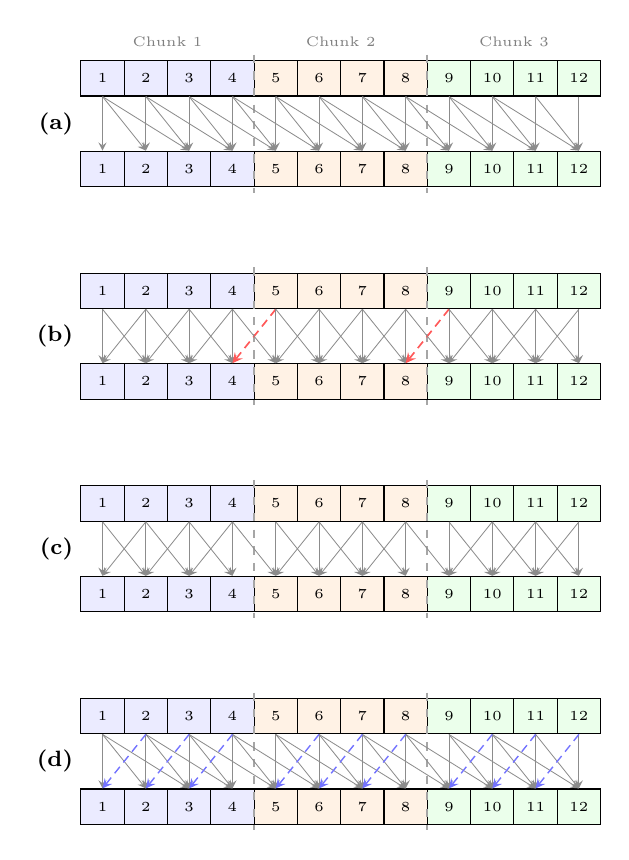
\begin{tikzpicture}[
    cell/.style={minimum width=0.55cm, minimum height=0.45cm, draw, inner sep=0pt, font=\tiny},
    c1/.style={cell, fill=blue!8},
    c2/.style={cell, fill=orange!10},
    c3/.style={cell, fill=green!8},
    arr/.style={->, >=stealth, line width=0.3pt, black!45},
    earr/.style={->, >=stealth, line width=0.5pt, blue!55, densely dashed},
    xarr/.style={->, >=stealth, line width=0.6pt, red!65, densely dashed},
    bnd/.style={thick, black!35, dashed},
]

\def\cw{0.55}
\def\rg{-1.15}

% ============================================================
%  (a) Causal convolution
% ============================================================
\def\yb{0}
\node[font=\footnotesize\bfseries, anchor=east] at (0.3, \yb+\rg/2) {(a)};

\foreach \i in {1,...,4}   { \node[c1] (ia\i) at (\i*\cw, \yb) {\i}; }
\foreach \i in {5,...,8}   { \node[c2] (ia\i) at (\i*\cw, \yb) {\i}; }
\foreach \i in {9,...,12}  { \node[c3] (ia\i) at (\i*\cw, \yb) {\i}; }
\foreach \i in {1,...,4}   { \node[c1] (oa\i) at (\i*\cw, \yb+\rg) {\i}; }
\foreach \i in {5,...,8}   { \node[c2] (oa\i) at (\i*\cw, \yb+\rg) {\i}; }
\foreach \i in {9,...,12}  { \node[c3] (oa\i) at (\i*\cw, \yb+\rg) {\i}; }

\draw[bnd] (4.5*\cw, \yb+0.3) -- (4.5*\cw, \yb+\rg-0.3);
\draw[bnd] (8.5*\cw, \yb+0.3) -- (8.5*\cw, \yb+\rg-0.3);

\node[font=\tiny, gray, anchor=south] at (2.5*\cw, \yb+0.28) {Chunk 1};
\node[font=\tiny, gray, anchor=south] at (6.5*\cw, \yb+0.28) {Chunk 2};
\node[font=\tiny, gray, anchor=south] at (10.5*\cw, \yb+0.28) {Chunk 3};

\draw[arr] (ia1.south) -- (oa1.north);
\draw[arr] (ia1.south) -- (oa2.north);
\draw[arr] (ia2.south) -- (oa2.north);
\draw[arr] (ia1.south) -- (oa3.north);
\draw[arr] (ia2.south) -- (oa3.north);
\draw[arr] (ia3.south) -- (oa3.north);
\draw[arr] (ia2.south) -- (oa4.north);
\draw[arr] (ia3.south) -- (oa4.north);
\draw[arr] (ia4.south) -- (oa4.north);
\draw[arr] (ia3.south) -- (oa5.north);
\draw[arr] (ia4.south) -- (oa5.north);
\draw[arr] (ia5.south) -- (oa5.north);
\draw[arr] (ia4.south) -- (oa6.north);
\draw[arr] (ia5.south) -- (oa6.north);
\draw[arr] (ia6.south) -- (oa6.north);
\draw[arr] (ia5.south) -- (oa7.north);
\draw[arr] (ia6.south) -- (oa7.north);
\draw[arr] (ia7.south) -- (oa7.north);
\draw[arr] (ia6.south) -- (oa8.north);
\draw[arr] (ia7.south) -- (oa8.north);
\draw[arr] (ia8.south) -- (oa8.north);
\draw[arr] (ia7.south) -- (oa9.north);
\draw[arr] (ia8.south) -- (oa9.north);
\draw[arr] (ia9.south) -- (oa9.north);
\draw[arr] (ia8.south) -- (oa10.north);
\draw[arr] (ia9.south) -- (oa10.north);
\draw[arr] (ia10.south) -- (oa10.north);
\draw[arr] (ia9.south) -- (oa11.north);
\draw[arr] (ia10.south) -- (oa11.north);
\draw[arr] (ia11.south) -- (oa11.north);
\draw[arr] (ia10.south) -- (oa12.north);
\draw[arr] (ia11.south) -- (oa12.north);
\draw[arr] (ia12.south) -- (oa12.north);

% ============================================================
%  (b) Standard non-causal convolution
% ============================================================
\def\yb{-2.7}
\node[font=\footnotesize\bfseries, anchor=east] at (0.3, \yb+\rg/2) {(b)};

\foreach \i in {1,...,4}   { \node[c1] (ib\i) at (\i*\cw, \yb) {\i}; }
\foreach \i in {5,...,8}   { \node[c2] (ib\i) at (\i*\cw, \yb) {\i}; }
\foreach \i in {9,...,12}  { \node[c3] (ib\i) at (\i*\cw, \yb) {\i}; }
\foreach \i in {1,...,4}   { \node[c1] (ob\i) at (\i*\cw, \yb+\rg) {\i}; }
\foreach \i in {5,...,8}   { \node[c2] (ob\i) at (\i*\cw, \yb+\rg) {\i}; }
\foreach \i in {9,...,12}  { \node[c3] (ob\i) at (\i*\cw, \yb+\rg) {\i}; }

\draw[bnd] (4.5*\cw, \yb+0.3) -- (4.5*\cw, \yb+\rg-0.3);
\draw[bnd] (8.5*\cw, \yb+0.3) -- (8.5*\cw, \yb+\rg-0.3);

\draw[arr] (ib1.south) -- (ob1.north);
\draw[arr] (ib2.south) -- (ob1.north);
\draw[arr] (ib1.south) -- (ob2.north);
\draw[arr] (ib2.south) -- (ob2.north);
\draw[arr] (ib3.south) -- (ob2.north);
\draw[arr] (ib2.south) -- (ob3.north);
\draw[arr] (ib3.south) -- (ob3.north);
\draw[arr] (ib4.south) -- (ob3.north);
\draw[arr]  (ib3.south) -- (ob4.north);
\draw[arr]  (ib4.south) -- (ob4.north);
\draw[xarr] (ib5.south) -- (ob4.north);
\draw[arr] (ib4.south) -- (ob5.north);
\draw[arr] (ib5.south) -- (ob5.north);
\draw[arr] (ib6.south) -- (ob5.north);
\draw[arr] (ib5.south) -- (ob6.north);
\draw[arr] (ib6.south) -- (ob6.north);
\draw[arr] (ib7.south) -- (ob6.north);
\draw[arr] (ib6.south) -- (ob7.north);
\draw[arr] (ib7.south) -- (ob7.north);
\draw[arr] (ib8.south) -- (ob7.north);
\draw[arr]  (ib7.south) -- (ob8.north);
\draw[arr]  (ib8.south) -- (ob8.north);
\draw[xarr] (ib9.south) -- (ob8.north);
\draw[arr] (ib8.south) -- (ob9.north);
\draw[arr] (ib9.south) -- (ob9.north);
\draw[arr] (ib10.south) -- (ob9.north);
\draw[arr] (ib9.south) -- (ob10.north);
\draw[arr] (ib10.south) -- (ob10.north);
\draw[arr] (ib11.south) -- (ob10.north);
\draw[arr] (ib10.south) -- (ob11.north);
\draw[arr] (ib11.south) -- (ob11.north);
\draw[arr] (ib12.south) -- (ob11.north);
\draw[arr] (ib11.south) -- (ob12.north);
\draw[arr] (ib12.south) -- (ob12.north);

% ============================================================
%  (c) Boundary-aware bidirectional convolution
% ============================================================
\def\yb{-5.4}
\node[font=\footnotesize\bfseries, anchor=east] at (0.3, \yb+\rg/2) {(c)};

\foreach \i in {1,...,4}   { \node[c1] (ic\i) at (\i*\cw, \yb) {\i}; }
\foreach \i in {5,...,8}   { \node[c2] (ic\i) at (\i*\cw, \yb) {\i}; }
\foreach \i in {9,...,12}  { \node[c3] (ic\i) at (\i*\cw, \yb) {\i}; }
\foreach \i in {1,...,4}   { \node[c1] (oc\i) at (\i*\cw, \yb+\rg) {\i}; }
\foreach \i in {5,...,8}   { \node[c2] (oc\i) at (\i*\cw, \yb+\rg) {\i}; }
\foreach \i in {9,...,12}  { \node[c3] (oc\i) at (\i*\cw, \yb+\rg) {\i}; }

\draw[bnd] (4.5*\cw, \yb+0.3) -- (4.5*\cw, \yb+\rg-0.3);
\draw[bnd] (8.5*\cw, \yb+0.3) -- (8.5*\cw, \yb+\rg-0.3);

\draw[arr] (ic1.south) -- (oc1.north);
\draw[arr] (ic2.south) -- (oc1.north);
\draw[arr] (ic1.south) -- (oc2.north);
\draw[arr] (ic2.south) -- (oc2.north);
\draw[arr] (ic3.south) -- (oc2.north);
\draw[arr] (ic2.south) -- (oc3.north);
\draw[arr] (ic3.south) -- (oc3.north);
\draw[arr] (ic4.south) -- (oc3.north);
\draw[arr] (ic3.south) -- (oc4.north);
\draw[arr] (ic4.south) -- (oc4.north);

\draw[arr] (ic4.south) -- (oc5.north);
\draw[arr] (ic5.south) -- (oc5.north);
\draw[arr] (ic6.south) -- (oc5.north);
\draw[arr] (ic5.south) -- (oc6.north);
\draw[arr] (ic6.south) -- (oc6.north);
\draw[arr] (ic7.south) -- (oc6.north);
\draw[arr] (ic6.south) -- (oc7.north);
\draw[arr] (ic7.south) -- (oc7.north);
\draw[arr] (ic8.south) -- (oc7.north);
\draw[arr] (ic7.south) -- (oc8.north);
\draw[arr] (ic8.south) -- (oc8.north);

\draw[arr] (ic8.south) -- (oc9.north);
\draw[arr] (ic9.south) -- (oc9.north);
\draw[arr] (ic10.south) -- (oc9.north);
\draw[arr] (ic9.south) -- (oc10.north);
\draw[arr] (ic10.south) -- (oc10.north);
\draw[arr] (ic11.south) -- (oc10.north);
\draw[arr] (ic10.south) -- (oc11.north);
\draw[arr] (ic11.south) -- (oc11.north);
\draw[arr] (ic12.south) -- (oc11.north);
\draw[arr] (ic11.south) -- (oc12.north);
\draw[arr] (ic12.south) -- (oc12.north);

% ============================================================
%  (d) BACON dual convolution = union of (a) and (c)
% ============================================================
\def\yb{-8.1}
\node[font=\footnotesize\bfseries, anchor=east] at (0.3, \yb+\rg/2) {(d)};

\foreach \i in {1,...,4}   { \node[c1] (id\i) at (\i*\cw, \yb) {\i}; }
\foreach \i in {5,...,8}   { \node[c2] (id\i) at (\i*\cw, \yb) {\i}; }
\foreach \i in {9,...,12}  { \node[c3] (id\i) at (\i*\cw, \yb) {\i}; }
\foreach \i in {1,...,4}   { \node[c1] (od\i) at (\i*\cw, \yb+\rg) {\i}; }
\foreach \i in {5,...,8}   { \node[c2] (od\i) at (\i*\cw, \yb+\rg) {\i}; }
\foreach \i in {9,...,12}  { \node[c3] (od\i) at (\i*\cw, \yb+\rg) {\i}; }

\draw[bnd] (4.5*\cw, \yb+0.3) -- (4.5*\cw, \yb+\rg-0.3);
\draw[bnd] (8.5*\cw, \yb+0.3) -- (8.5*\cw, \yb+\rg-0.3);

% Causal arrows (same as panel a) -- solid gray
\draw[arr] (id1.south) -- (od1.north);
\draw[arr] (id1.south) -- (od2.north);
\draw[arr] (id2.south) -- (od2.north);
\draw[arr] (id1.south) -- (od3.north);
\draw[arr] (id2.south) -- (od3.north);
\draw[arr] (id3.south) -- (od3.north);
\draw[arr] (id2.south) -- (od4.north);
\draw[arr] (id3.south) -- (od4.north);
\draw[arr] (id4.south) -- (od4.north);
\draw[arr] (id3.south) -- (od5.north);
\draw[arr] (id4.south) -- (od5.north);
\draw[arr] (id5.south) -- (od5.north);
\draw[arr] (id4.south) -- (od6.north);
\draw[arr] (id5.south) -- (od6.north);
\draw[arr] (id6.south) -- (od6.north);
\draw[arr] (id5.south) -- (od7.north);
\draw[arr] (id6.south) -- (od7.north);
\draw[arr] (id7.south) -- (od7.north);
\draw[arr] (id6.south) -- (od8.north);
\draw[arr] (id7.south) -- (od8.north);
\draw[arr] (id8.south) -- (od8.north);
\draw[arr] (id7.south) -- (od9.north);
\draw[arr] (id8.south) -- (od9.north);
\draw[arr] (id9.south) -- (od9.north);
\draw[arr] (id8.south) -- (od10.north);
\draw[arr] (id9.south) -- (od10.north);
\draw[arr] (id10.south) -- (od10.north);
\draw[arr] (id9.south) -- (od11.north);
\draw[arr] (id10.south) -- (od11.north);
\draw[arr] (id11.south) -- (od11.north);
\draw[arr] (id10.south) -- (od12.north);
\draw[arr] (id11.south) -- (od12.north);
\draw[arr] (id12.south) -- (od12.north);

% Extra arrows from bidirectional group (right-context within chunk) -- dashed blue
% Chunk 1: output 1 gets +1 from bidir; output 2 gets +1; output 3 gets +1; output 4 at edge gets nothing extra
\draw[earr] (id2.south) -- (od1.north);
\draw[earr] (id3.south) -- (od2.north);
\draw[earr] (id4.south) -- (od3.north);
% Chunk 2: output 5 gets +1; output 6 gets +1; output 7 gets +1; output 8 at edge gets nothing extra
\draw[earr] (id6.south) -- (od5.north);
\draw[earr] (id7.south) -- (od6.north);
\draw[earr] (id8.south) -- (od7.north);
% Chunk 3: output 9 gets +1; output 10 gets +1; output 11 gets +1; output 12 at edge gets nothing extra
\draw[earr] (id10.south) -- (od9.north);
\draw[earr] (id11.south) -- (od10.north);
\draw[earr] (id12.south) -- (od11.north);

\end{tikzpicture}

\caption{Input-to-output dependencies of a 1D convolution (kernel size~3,
chunk size~4) for 12 frames across three chunks (dashed boundaries).
\textbf{(a)}~Causal convolution: each output depends only on current and past
frames.
\textbf{(b)}~Standard non-causal convolution (not streaming-safe): \textcolor{red!65}{red dashed} arrows
mark dependencies on frames from future chunks.
\textbf{(c)}~Boundary-aware bidirectional convolution: left context crosses
chunk boundaries freely, right context is confined within each chunk.
\textbf{(d)}~BACON (union of (a) and~(c)): solid arrows show the causal
group's dependencies; \textcolor{blue!55}{blue dashed} arrows show the additional
within-chunk right context contributed by the bidirectional group.
Positions at right chunk edges (frames 4, 8, 12) receive no extra right
context from the bidirectional group, but the causal group still provides
full backward context at those positions.}
\label{fig:chunk_conv_deps}
\end{figure}

%----------------------------------------------------------------------
\section{Experiments}
\label{sec:experiments}

We use NeMo \cite{kuchaiev2019nemo} toolkit to conduct all our experiments. 
All experiments use a FastConformer encoder, where 8$\times$ subsampling is first performed on 80-dimension Mel-spectrogram features with causal subsampling; then the subsampled representation goes through 17 layers of Conformer blocks, with $d_{\text{model}}{=}512$ and convolution kernel size $k{=}9$. The streaming chunk size is $C{=}14$ subsampled frames, equivalent to $14 \times 80 = 1120$\,ms of speech. Chunked attention is configured so that each frame can attend to any frame in the current chunk as well as 5 chunks in the past. These are all standard configurations for NeMo's FastConformer-Large, with full details available at \url{https://github.com/NVIDIA-NeMo/NeMo/blob/main/examples/asr/conf/fastconformer/cache_aware_streaming/fastconformer_transducer_bpe_streaming.yaml}.

We use two basic model architectures for training. 1. A standard RNN-T~\cite{graves2012sequence} model and 2. A Chunk-wise Attention Transducer (CHAT)~\cite{xu2026chunk}. 
For all models and datasets, we train and compare two models with identical architecture and hyper-parameters, except one with causal convolution in conformers, and the other with the BACON architecture in conformer. 
All models are trained with fast-emit lambda=0.005.
We evaluate on three tasks: speech recognition on LibriSpeech~\cite{panayotov2015librispeech}, multi-speaker speech
recognition on Fisher~\cite{cieri2004fisher},
and speech-to-text translation on CoVoST~\cite{wang2021covost2} and MuST-C~\cite{di-gangi-etal-2019-must}. For all models, we average the five best checkpoints before evaluation.

\subsection{Speech Recognition}
\label{subsec:libri}

We train our LibriSpeech model from scratch using the full 960-hour training
set. For text tokenization, we train a SentencePiece~\cite{kudo2018sentencepiece}
model with a vocabulary size of 1024.

\begin{table}[h]
\centering
\caption{WER~(\%) on LibriSpeech. BACON improves over the causal baseline
across conditions, with the largest gains on \texttt{test-other}.}
\label{tab:libri_wer}
\begin{tabular}{llcc}
\toprule
\textbf{Family} & \textbf{Conv.\ mode} & \textbf{test-clean}$\downarrow$ & \textbf{test-other}$\downarrow$ \\
\midrule
\textsc{rnn-t} & Causal & \textbf{3.33} & 8.72 \\
\textsc{rnn-t} & BACON  & 3.39 & \textbf{8.52} \\
\midrule
\textsc{chat} & Causal & 3.26 & 8.44 \\
\textsc{chat} & BACON  & \textbf{3.13} & \textbf{7.91} \\

\bottomrule
\end{tabular}
\end{table}


As shown in Table 1, on LibriSpeech \texttt{test-clean}, BACON and Causal achieve similar accuracy, which is expected given the relatively clean conditions. 
On the more challenging \texttt{test-other} set, BACON yields larger gains, especially for \textsc{chat}, where it improves WER by 0.53 absolute over the causal baseline, a -6.3\% relative WER reduction.

\subsection{Multi-Speaker ASR}
\label{subsec:multispk}

To evaluate generality, we further assess BACON on a two-speaker ASR task.
Following~\cite{wang2024resource}, we insert special speaker
tokens (\texttt{<spk1>}, \texttt{<spk2>}) at each speaker change to training text in order to model
speaker turns explicitly. We use segment-level speaker annotations and train onw
Fisher, which contains approximately 2,000 hours of
labeled two-speaker conversational speech. Encoder parameters are initialized
from checkpoints pre-trained for approximately 10k steps on LibriSpeech in the
corresponding training mode. We report concatenated minimum-permutation word
error rate (cpWER)~\cite{watanabe2020chime}, the standard metric for
multi-speaker ASR.

\begin{table}[h]
\centering
\caption{cpWER~(\%) on 2-speaker ASR. All models are CHAT-120M with chunk
configuration [70,13] and 300K training steps.}
\label{tab:multispk}
\begin{tabular}{lcc}
\toprule
\textbf{Conv.\ mode} & \textbf{cpWER (\%)}$\downarrow$ \\
\midrule
Causal (baseline)      & 27.41 \\
BACON                  & \textbf{27.14} \\
\bottomrule
\end{tabular}
\end{table}

Table 2 demonstrates that BACON reduces cpWER from 27.41\% to 27.14\%, achieving a 0.27\% absolute improvement. Notably, multi-speaker ASR involves rapid speaker alternation where short-range within-chunk context is especially informative for disambiguating overlapping or adjacent speech, making it a particularly natural fit for BACON's wider receptive field.
\subsection{Speech Translation}
\label{subsec:ast}

We evaluate English-to-German speech-to-text translation across both families, reporting BLEU on MuST-C~(\textsc{must-c}) and CoVoST~2~(\textsc{covost}) test sets. 
Models are trained on Mozilla Common Voice~\cite{ardila2020common}, Multilingual LibriSpeech~\cite{pratap2020mls}, and VoxPopuli~\cite{wang2021voxpopuli}.
Encoders are initialized from checkpoints pre-trained for approximately 10k steps on LibriSpeech in the corresponding convolution mode. 
For tokenization, we use a SentencePiece model with a 16k vocabulary.

\begin{table}[h]
\centering
\caption{BLEU on English-to-German AST. BACON improves over the causal
baseline in both model families on both evaluation sets.}
\label{tab:chunk_conv_bleu}
\begin{tabular}{llcc}
\toprule
\textbf{Family} & \textbf{Conv.\ mode} & \textbf{MuST-C}$\uparrow$ & \textbf{CoVoST}$\uparrow$ \\

\midrule
\textsc{rnn-t} & Causal   & 24.43 & 33.60 \\
\textsc{rnn-t} & BACON    & \textbf{25.21} & \textbf{33.85} \\
\midrule
\textsc{chat} & Causal   & 27.97 & 36.50 \\
\textsc{chat} & BACON    & \textbf{28.65} & \textbf{36.72} \\
\bottomrule
\end{tabular}
\end{table}

As detailed in Table 3, BACON improves over the causal baseline on both evaluation sets in both families:
+0.22 BLEU on \textsc{covost} for \textsc{chat} and +0.25 for \textsc{rnn-t},
with larger \textsc{must-c} gains of +0.68 and +0.78, respectively.
The improvement is consistent across both families and both evaluation sets, confirming that the
benefit derives from the wider receptive field rather than any
architecture-specific interaction.




%----------------------------------------------------------------------
\section{Analysis}
\label{sec:analysis}

\subsection{Importance of dual-mode design}
\label{subsec:analysis-zero-vs-split}

A natural alternative to BACON's split design is to make \emph{all} channels
bidirectional (\textbf{all-bidir}). Tables~\ref{tab:analysis-zero-vs-split-libri}
and~\ref{tab:analysis-zero-vs-split-ast} compare all-bidir and BACON on
LibriSpeech and AST respectively.

\begin{table}[h]
\centering
\caption{All-bidir vs.\ BACON on LibriSpeech (WER\,\%).}
\label{tab:analysis-zero-vs-split-libri}
\begin{tabular}{llcc}
\toprule
\textbf{Family} & \textbf{Conv.\ mode} & \textbf{test-clean}$\downarrow$ & \textbf{test-other}$\downarrow$ \\
\midrule
\textsc{chat} & all-bidir  & 3.23 & 8.24 \\
\textsc{chat} & BACON & \textbf{3.13} & \textbf{7.91} \\
\midrule
\textsc{rnn-t} & all-bidir  & 3.40 & 8.79 \\
\textsc{rnn-t} & BACON & \textbf{3.39} & \textbf{8.52} \\
\bottomrule
\end{tabular}
\end{table}

\begin{table}[h]
\centering
\caption{All-bidir vs.\ BACON on AST (BLEU).}
\label{tab:analysis-zero-vs-split-ast}
\begin{tabular}{llcc}
\toprule
\textbf{Family} & \textbf{Conv.\ mode} & \textbf{MuST-C}$\uparrow$ & \textbf{CoVoST}$\uparrow$ \\
\midrule
\textsc{chat} & all-bidir  & \textbf{28.65} & 36.32 \\
\textsc{chat} & BACON & \textbf{28.65} & \textbf{36.72} \\
\midrule
\textsc{rnn-t} & all-bidir  & 24.60 & 33.43 \\
\textsc{rnn-t} & BACON & \textbf{25.21} & \textbf{33.85} \\
\bottomrule
\end{tabular}
\end{table}

BACON consistently and substantially outperforms all-bidir. On LibriSpeech
\texttt{test-other}, BACON beats all-bidir by $-$0.33 WER for \textsc{chat} and
$-$0.27 for \textsc{rnn-t}. On \textsc{covost}, BACON leads by +0.40 BLEU
(\textsc{chat}) and +0.42 (\textsc{rnn-t}).

Critically, for \textsc{rnn-t} on LibriSpeech, all-bidir \emph{degrades} relative
to the causal baseline (8.79\% vs.\ 8.72\%), whereas BACON improves it
(8.52\%). 
%The same pattern appears on multi-speaker ASR: all-bidir increases cpWER
% to 27.58\% (worse than the 27.41\% baseline), while BACON improves it to
% 27.14\%. 
This is a direct consequence of chunk boundary effects: when all
channels are bidirectional, positions at right chunk edges see fewer real
inputs across every channel simultaneously, reducing the effective receptive
field. The causal group in BACON acts
as a boundary stabilizer, always providing $k$ real past inputs regardless
of position within the chunk. For those comparisons, we conclude that the split design is
not merely helpful but necessary for robust and consistent gains.



\subsection{Convolution Benefits from Right Context Independently of Attention}
\label{subsec:analysis-fullctx}

In a chunk-based Conformer, both attention and convolution operate on the same
frames, and within each chunk the attention module already has bidirectional
access up to the chunk boundary. One might therefore wonder whether the convolution module gains
anything from right context that attention has not already captured.
To test this, we construct an extreme upper bound: we train
full-context Conformer-Transducers on LibriSpeech where self-attention is
\emph{completely unrestricted}, where every frame can attend to the entire utterance.
In this setting, attention has strictly more context than in any streaming
configuration. We compare two otherwise identical models that differ only in
convolution mode: causal vs.\ non-causal (symmetric).

\begin{table}[h]
\centering
\caption{WER~(\%) on LibriSpeech \texttt{test-other} for full-context
Conformers (unrestricted attention) with causal vs.\ non-causal convolution.}
\label{tab:analysis-fullctx}
\begin{tabular}{lc}
\toprule
\textbf{Convolution} & \textbf{test-other}$\downarrow$ \\
\midrule
Causal      & 8.16 \\
Non-causal  & \textbf{7.23} \\
\bottomrule
\end{tabular}
\end{table}

As shown in Table 6, even with full-utterance attention, non-causal convolution reduces WER by 0.93
absolute (8.16\%~$\rightarrow$~7.23\%, an 11.4\% relative improvement). This
demonstrates that convolution and attention capture complementary structure:
the convolution module extracts local acoustic patterns that attention does not
subsume, even when attention has access to the entire sequence. Restricting
convolution to past-only context therefore leaves significant accuracy on the
table regardless of how much context attention provides---directly motivating
BACON's design.

\subsection{Impact on Latency}

In chunk-based streaming, the encoder buffers input frames until a full chunk
of $C$ frames has been accumulated before processing begins. Consequently,
regardless of which frame within the chunk is responsible for a particular
token emission, the token can only be produced after the last frame of the
chunk has arrived. The effective emission time of any token emitted during
chunk~$i$ is therefore
\begin{equation}
    t_{\text{emit}}(i) = (i+1) \cdot C \cdot \Delta + \delta,
    \label{eq:emit-time}
\end{equation}
where $\Delta$ is the frame duration and $\delta$ is a processing
delay shared across all models, which we assume is constant. The true latency for a token corresponding to word~$j$ with
ground-truth timestamp~$\tau_j$ is
$\ell_j = t_{\text{emit}}(i_j) - \tau_j$,
where $i_j$ is the chunk in which the token is emitted. Averaging over all
$N$ emitted tokens:

\begin{equation}
    \begin{aligned}
        \bar{\ell} &= \frac{1}{N}\sum_{j=1}^{N} \bigl[(i_j+1)\cdot C\cdot\Delta + \delta - \tau_j\bigr] \\
                   &= (C\cdot\Delta) \bar{\imath} + (C\cdot\Delta + \delta) - \bar{\tau},
    \end{aligned}
    \label{eq:avg-latency}
\end{equation}

where $\bar{\imath} = \frac{1}{N}\sum_j i_j$ is the average chunk index of all
emissions and $\bar{\tau} = \frac{1}{N}\sum_j \tau_j$ is the average
ground-truth timestamp. When comparing two models~A and~B evaluated on the
same utterances, the timestamp term $\bar{\tau}$ and the constant
$(C\cdot\Delta + \delta)$ cancel:
\begin{equation}
    \bar{\ell}^{A} - \bar{\ell}^{B} = (C\cdot\Delta)\;(\bar{\imath}^{A} - \bar{\imath}^{B}).
    \label{eq:latency-diff}
\end{equation}
Thus the difference in average emission chunk index between two models is
proportional to their difference in average latency, with the proportionality
constant $C\cdot\Delta$ determined solely by the chunk configuration. This
allows us to compare latency across convolution modes without requiring
time-stamped reference transcripts: a lower $\bar{\imath}$ directly implies lower
latency.

\begin{table}[h]
\centering
\caption{Average emission chunk index ($\bar{\imath}$) on LibriSpeech
\texttt{test-other}. Lower is earlier (lower latency).}
\label{tab:latency}
\begin{tabular}{llc}
\toprule
\textbf{Family} & \textbf{Conv.\ mode} & $\bar{\imath}$ $\downarrow$ \\
\midrule
\textsc{rnn-t} & Causal & 4.07 \\
\textsc{rnn-t} & BACON  & 4.05 \\
\midrule
\textsc{chat} & Causal & 4.16 \\
\textsc{chat} & BACON  & 4.13 \\
\bottomrule
\end{tabular}
\end{table}

We measure the average emission chunk index of different models on
LibriSpeech \texttt{test-other}. Table~\ref{tab:latency} shows that BACON's
average emission chunk index is
slightly \emph{lower} than the causal baseline in both model families,
indicating that BACON does not increase latency and in fact emits tokens
marginally earlier on average. 
While the difference is small, it is consistent
with BACON's wider receptive field: by incorporating within-chunk right
context, the encoder produces more informative frame representations and can
emit tokens slightly earlier than the causal baseline. Combined with
the accuracy gains reported in
Sections~\ref{subsec:libri}--\ref{subsec:multispk}, this confirms that BACON
improves recognition quality while maintaining  emission latency.

%----------------------------------------------------------------------
\section{Conclusion}
\label{sec:conclusion}

We show that causal convolution in chunk-based streaming Conformers is
unnecessarily restrictive, and we propose BACON, which splits depthwise
channels into a causal group and a boundary-aware bidirectional group. This
widens receptive field without changing model architecture or parameter count.
Across three tasks and two model families, BACON improves accuracy while
maintaining (and in our measurements, slightly reducing) emission latency. For
future work, we plan to apply BACON to larger-scale datasets and other
speech-to-text tasks, including streaming speech LLM systems.

%----------------------------------------------------------------------
\section{Generative AI Use Disclosure}
\label{sec:genai}

Generative AI tools were used solely to assist with editing and polishing the
writing of this paper (e.g., grammar, phrasing, and clarity). They were not
used to generate any major part of the paper's research content, including the
ideas, methodology, experiments, analysis, or results.

\bibliographystyle{IEEEtran}
\bibliography{references}

\end{document}